% A Few Tokens Are Sometimes Enough: Steering Vectors from a Jacobian Lens
% Reconstructed from the submitted PDF (102_Extracting_Steering_Vector.pdf).
% Compile with XeTeX via tectonic:  tectonic main.tex
\documentclass{article}

% Camera-ready version
\usepackage[dblblindworkshop, final]{neurips_2026}

% ---------------------------------------------------------------- fonts (XeTeX)
\usepackage{fontspec}
\setmainfont{Times New Roman}
% Chinese tokens (the submission used STSongti-SC-Regular = "Songti SC",
% scaled to 0.92: measured from the glyph boxes in the submitted PDF)
\newfontfamily\zhfont{Songti SC}[Scale=0.92]
\newcommand{\zh}[1]{{\zhfont #1}}

% ---------------------------------------------------------------- packages
\usepackage{hyperref}       % hyperlinks
\usepackage{url}            % simple URL typesetting
\usepackage{booktabs}       % professional-quality tables
\usepackage{amsmath}
\usepackage{amsfonts}       % blackboard math symbols
\usepackage{nicefrac}       % compact symbols for 1/2, etc.
\usepackage{microtype}      % microtypography
\usepackage[table]{xcolor}  % colors (+ colortbl)
\usepackage{array}
\usepackage{multirow}
\usepackage{graphicx}
\usepackage{listings}
\usepackage{caption}

% ---------------------------------------------------------------- colours
% table shading: green = ours ahead by > 0.10, red = fitted ahead by > 0.10
\definecolor{posgreen}{rgb}{0.88,1,0.88}   % #e0ffe0
\definecolor{negred}{rgb}{1,0.88,0.88}     % #ffe0e0
\definecolor{ctrlgrey}{gray}{0.5}          % #808080, J=I and random columns
% listings
\definecolor{lstbg}{gray}{0.98}
\definecolor{lstframe}{gray}{0.8}
\definecolor{lstkw}{rgb}{0,0,0.8}
\definecolor{lststr}{rgb}{0.7,0,0}
\definecolor{lstcmt}{rgb}{0,0.5,0}

% Appendix F: intervals in grey brackets, and the four cases as shaded letters (hues as in Fig. F1)
\newcommand{\ci}[2]{{\color{ctrlgrey}\tiny[#1,\,#2]}}
\definecolor{caseJc}{HTML}{D6E5F8}\definecolor{caseUc}{HTML}{FBDCCD}
\definecolor{caseEc}{HTML}{CFEFE3}\definecolor{caseSc}{HTML}{ECEBE7}
\newcommand{\caseJ}{\cellcolor{caseJc}J}\newcommand{\caseU}{\cellcolor{caseUc}U}
\newcommand{\caseE}{\cellcolor{caseEc}E}\newcommand{\caseS}{\cellcolor{caseSc}S}
\newcommand{\caseN}{{\color{ctrlgrey}--}}
\newcommand{\FGapMean}{0.02}
\newcommand{\FGapMax}{0.27}
\newcommand{\FSeedSDMedian}{0.03}
\newcommand{\FSeedSDMax}{0.52}
\newcommand{\FCIHalfMedian}{0.06}
\newcommand{\FNModels}{8}
\newcommand{\FNMix}{6}
\newcommand{\FNDepth}{6}
\newcommand{\FJudgeAgreeMin}{0.77}
\newcommand{\FJudgeAgreeMax}{0.95}
\newcommand{\FMixWins}{12}
\newcommand{\FMixCells}{46}
\newcommand{\FCosMax}{0.30}
\newcommand{\FCosMedian}{0.08}
\newcommand{\FCaseJ}{7}
\newcommand{\FCaseU}{14}
\newcommand{\FCaseE}{5}
\newcommand{\FCaseS}{19}
\newcommand{\FCaseN}{17}
\newcommand{\FJudgeHedgeU}{5}
\newcommand{\FJudgeHedgeN}{6}
\newcommand{\FJudgeSycoU}{6}
\newcommand{\FJudgeSycoN}{6}
\newcommand{\FKwHedgeN}{7{,}403}
\newcommand{\FKwHedgeCoh}{38\%}
\newcommand{\FKwHedgeIncoh}{33\%}
\newcommand{\FKwHedgeNot}{29\%}
   % numbers quoted from Appendix F (generated by appendix.py)
\newcommand{\pos}{\cellcolor{posgreen}}
\newcommand{\negc}{\cellcolor{negred}}
\newcommand{\dlt}[1]{{\scriptsize(#1)}}
\newcolumntype{g}{>{\color{ctrlgrey}}r}

% Emoji placeholder. The submitted PDF prints the literal text "[emoji]" for
% every emoji concept token in Table 3; the actual emoji are not recoverable
% from the PDF.  TODO: replace with the real emoji tokens.
% In the submission the placeholder is set at 8pt (\footnotesize), larger than the
% surrounding 7pt token list; reproduced here.
\newcommand{\emojiph}[1][]{{\footnotesize\texttt{[emoji]}}}

\lstset{
  language=Python,
  basicstyle=\ttfamily\scriptsize,
  keywordstyle=\color{lstkw}\bfseries,
  keywordstyle={[2]\color{lstkw}\bfseries},
  stringstyle=\color{lststr},
  commentstyle=\color{lstcmt}\itshape,
  backgroundcolor=\color{lstbg},
  frame=single,
  rulecolor=\color{lstframe},
  xleftmargin=3pt,
  framexleftmargin=3pt,
  belowskip=\smallskipamount,
  showstringspaces=false,
  captionpos=t,
  morekeywords={True,False},
}

\title{A Few Tokens Are Sometimes Enough: Steering Vectors from a Jacobian Lens}
\workshoptitle{Neural Network Artifacts as a New Data Modality}

% Correspondence email: blue, clickable, without hyperref's link box.
\DeclareRobustCommand{\correspondenceemail}{{\hypersetup{pdfborder={0 0 0}}\href{mailto:darshanm@signallabs.ai}{\textcolor{blue}{darshanm@signallabs.ai}}}}
\author{%
  Darshan Makwana \\
  Signal Labs \\
  \And
  Naman Garg \\
  Signal Labs \\
}

\begin{document}

\maketitle
{\renewcommand{\thefootnote}{}\footnotetext{Correspondence to: Darshan Makwana (\correspondenceemail)}}  % unmarked footnote

\begin{abstract}
  In this work, we explore the idea of deriving steering vectors from a published Jacobian lens rather than from behavioural examples, as an exploratory extension of the lens's token-level steering. To that end, we run the lens backwards: the unembedding rows of a few concept tokens are pulled back through the lens Jacobian to the activation direction that raises their lens logit, contrasted against counter-tokens, and averaged. We evaluate the resulting direction against a difference-in-means vector fitted on the model over 8 behaviours on Qwen3-1.7B and show that it matches the fitted vector on behaviours that amount to a preference over word choice. Finally, we present results suggesting two kinds of failure: one where the subspace the concept tokens can reach contains a working direction that our average misses, and one where it does not.
\end{abstract}

% =====================================================================
\section{Introduction}

Steering vectors are directions added to the residual stream of a language model that shift its behaviour, for instance towards answering in capitals or towards refusing. They are usually obtained by contrasting activations on paired prompts and taking a difference of means \citep{turner2023actadd,rimsky2024caa,zou2023repe}, which requires a dataset, a forward pass per example, and a choice of contrast. \citet{arditi2024refusal} showed that refusal in particular is mediated by a single such direction. Separately, a family of lenses decodes intermediate activations into tokens: the logit lens \citep{nostalgebraist2020logitlens}, the tuned lens \citep{belrose2023tuned}, and most recently the Jacobian lens \citep{gurnee2026workspace}, a matrix fitted once per layer whose lens vectors make up what that paper calls the J-space. Pre-fitted lenses are now published for over 40 open-weight models \citep{neuronpedia2026jlens}. The workspace paper swaps the lens vector of one concept for another (spider for ant) to steer the output, and \citet{gong2026firsttoken} extend the readout to multi-token concepts.

A lens maps activations to tokens and a steering vector runs the other way, so the natural question is whether a published lens can be inverted into a steering vector from concept tokens alone. The workspace paper already does this for a single concept. In this work, we extend the idea to behaviours that no single token names, such as hedging or answering in French, and study where the extension succeeds and where it fails. We present this as an exploratory study on one model and one lens family, with further experiments on seven more models in Appendix~\ref{app:further}. We (1) construct behavioural steering vectors from a published Jacobian lens and a list of concept tokens, with no behavioural examples and no gradients (the lens itself is corpus-fitted), and benchmark them against fitted vectors over 8 behaviours; (2) show that the construction is competitive with the fitted vector where the behaviour is a preference over word choice, and that for two of these behaviours the unembedding geometry alone suffices; and (3) present two diagnostics, a lens readout and an oracle projection, whose results separate two failure modes: an \emph{estimator} failure, where the subspace the concept tokens span contains a working direction that our average misses (French), and a \emph{subspace} failure, where it does not (refusal, pirate register).

% =====================================================================
\section{Background}

\paragraph{Steering vectors.}
Given a direction $d_\ell$ at layer $\ell$, steering adds $\alpha d_\ell$ to the residual stream at every position during generation. The standard recipe, difference-in-means or contrastive activation addition, runs the model on prompts under a positive and a negative condition and takes the difference of mean activations \citep{rimsky2024caa}. A stronger published alternative for refusal is \emph{abliteration}: \citet{arditi2024refusal} orthogonalise the weights that write into the residual stream against the refusal direction, so the difference between an abliterated checkpoint and its base model, a task vector in the sense of \citet{ilharco2023task}, is that direction applied at every layer.

\begin{figure}[t]
  \centering
  \includegraphics[width=0.8\linewidth]{figures/fig1_pca.png}
  \caption{Lens inversion on capitalisation. Every lowercase token in the vocabulary of Qwen3-1.7B that has a capitalised twin (\texttt{and} and \texttt{AND}) is pulled back through the layer-13 lens to the activation the lens would decode as that token; grey points are the lowercase tokens and orange points their capitalised twins, shown in the top two principal components. Arrows join twenty labelled pairs and all point the same way. The dashed line is a published capitalisation steering vector, fitted from a model finetuned to answer in capitals, projected onto the same components: the direction shared by the pairs aligns with the fitted steering direction in these components.}
  \label{fig:pca}
\end{figure}

\paragraph{Jacobian lens.}
The Jacobian lens \citep{gurnee2026workspace} estimates the average linearisation of the network from layer $\ell$ to the final layer $L$ and decodes through the model's own final norm and unembedding $W_U$,
\begin{equation}
  J_\ell \;=\; \mathbb{E}_x\!\left[\frac{\partial h_L(x)}{\partial h_\ell(x)}\right],
  \qquad
  \mathrm{lens}_\ell(h) \;=\; W_U\big(g \odot \mathrm{RMSNorm}(J_\ell h)\,\big),
  \label{eq:lens}
\end{equation}
where $g$ is the gain of the final norm. $J_\ell$ is estimated over a corpus of prompts and is expensive to fit, but the fitted matrices are published. The only property we rely on is that $J_\ell$ is linear.

% =====================================================================
\section{Method}

\paragraph{Intuition.}
By Eq.~\ref{eq:lens}, every token $t$ has a direction at layer $\ell$ that most raises its lens logit, its pull-back $J_\ell^\top (g \odot u_t)$. For two tokens that share a meaning and differ in one property, the difference of their pull-backs is the residual change that produces that property. A behaviour that is a preference in word choice is a collection of such contrasts (a word against its capitalised form, a neutral word against a hedge), and averaging over them cancels what is specific to each word and keeps the behaviour. Figure~\ref{fig:pca} checks this on capitalisation, where the vocabulary supplies the pairs: the lowercase tokens form one cloud, their capitalised twins another, the arrows joining pairs point the same way, and that direction coincides with a published capitalisation steering vector fitted from activations. For behaviours without natural twins, the construction below uses a hand-chosen counter-token and averages over sampled subsets of contrasts.

\paragraph{Lens inversion.}
Let $u_t$ be the unembedding row of token $t$. Reading Eq.~\ref{eq:lens} backwards, the layer-$\ell$ activation that most raises the lens logit of $t$ at fixed norm is $J_\ell^\top (g \odot u_t)$. Since a behaviour is not a single token, we contrast a set of concept tokens $P$ with an index-matched set of counter-tokens $N$ (\texttt{cannot} against \texttt{can}, \texttt{THE} against \texttt{the}), sample $k$ subsets $S_i$ of size $c$, and average the normalised pull-backs:
\begin{equation}
  d_\ell \;=\; \mathrm{unit}\!\left(\sum_{i=1}^{k} \mathrm{unit}\Big(J_\ell^\top \Big(g \odot \big(\bar u_{P(S_i)} - \bar u_{N(S_i)}\big)\Big)\Big)\right),
  \qquad
  \bar u_A = \tfrac{1}{|A|}\!\sum_{t \in A}\!u_t .
  \label{eq:inv}
\end{equation}
The inner normalisation is necessary because unembedding rows differ in norm by more than an order of magnitude and a few high-norm tokens otherwise dominate the mean. We use $c = 3$ and $k = 20$; in pilot runs neither mattered much, nor did replacing the counter-tokens by the vocabulary mean. Everything in Eq.~\ref{eq:inv} is offline: the lens, the unembedding, the norm gain and a list of tokens suffice; the only use of the model is one batched forward pass over the evaluation prompts to measure the injection scale below.

\paragraph{Controls.}
Replacing $J_\ell$ with the identity in Eq.~\ref{eq:inv} yields the $J{=}I$ control, which isolates what the fitted lens contributes over the geometry of the unembedding alone. A norm-matched Gaussian direction serves as a random control.

\paragraph{Scaling and injection.}
We add $\alpha \rho_\ell d_\ell$ to the output of block $\ell$ at every position, where $\rho_\ell$ is the mean $L_2$ norm of the residual stream at that layer over the last prompt position of the evaluation prompts, so that $\alpha$ is expressed in units of the layer's own scale.

\paragraph{Diagnostics.}
Two tools are used to analyse the resulting directions. The \emph{lens readout} decodes a direction through Eq.~\ref{eq:lens} and lists its top tokens, which shows what the direction disposes the model to say. The \emph{oracle projection} tests whether a behaviour is reachable from the concept tokens at all: whatever weights Eq.~\ref{eq:inv} uses, $d_\ell$ lies in $V = \mathrm{span}\{J_\ell^\top (g \odot (u_p - u_n))\}$ over the concept pairs, a subspace of dimension at most the number of pairs. We project the fitted direction, which is known to induce the behaviour, orthogonally onto $V$ and steer with the projection. The projection is one element of $V$ and not a maximum over it, so a failure is evidence of unreachability rather than proof.

% =====================================================================
\section{Experiment Setup}

All experiments use Qwen3-1.7B with its published Jacobian lens; we fit no lenses. Directions are injected at depth $0.55L$, which is layer 15 of 28. We consider 8 behaviours, ordered from lexical to dispositional before any experiment was run: capitalisation, answering in French, emoji use, pirate register, hedging, sycophantic agreement, refusing harmless requests, and extreme brevity. Each behaviour has a hand-written list of concept tokens, an index-matched counter-list, an instruction pair for the fitted baseline, and a functional test (Appendix~\ref{app:behaviours}).

\paragraph{Baselines.}
The fitted baseline is difference-in-means over paired instructed generations, averaged over the model's own continuations.\footnote{Averaging at the last prompt token instead mostly recovers the difference between the two instruction strings.} Two published steering artifacts are included where they apply: a capitalisation vector fitted from a model finetuned to answer in capitals, and a refusal direction recovered from \texttt{mlabonne/Qwen3-1.7B-abliterated} by differencing it against its base (Appendix~\ref{app:impl}).

\paragraph{Metrics.}
The \emph{behaviour rate} is a functional test of the behaviour itself, for instance whether the answer is in French or whether it refuses (Appendix~\ref{app:behaviours}). For hedging and capitalisation the test is itself lexical (hedge-word rate, share of capitalised words), which is close to what Eq.~\ref{eq:inv} optimises, so those rows test only the lexical claim. The sycophancy test is also keyword-based and may reward affirmation words rather than agreement with a false premise.

\paragraph{Quality gate and protocol.}
A direction pushed hard enough moves a keyword metric while producing degenerate text, so every reported number is the peak over 11 coefficients ($0.025$ to $1.2$) whose completions pass a gate, selected and reported on the same prompts. This in-sample selection is exploratory and may overstate rates on so few prompts. In the experiments of Appendix~\ref{app:further}, selecting the coefficient on held-out prompts instead lowers rates by \FGapMean\ on average and by at most \FGapMax. Completions are judged individually on five signals ($n$-gram repetition, loop score, out-of-script characters, punctuation share and long-token share) with thresholds calibrated on hand-read cases; a degenerate completion scores zero and a cell is rejected once more than 30\% of it is degenerate (Appendix~\ref{app:gate}). Decoding is greedy over 32 prompts (16 for sycophancy) and three seeds, where the seed affects only the sampled token subsets and the random control. The oracle probe is a separate single-seed run, so its \emph{ours} column differs from Table~\ref{tab:main}, most for sycophancy with its 16 prompts. The published capitalisation vector was fitted for layer 13 and is compared there (Appendix~\ref{app:impl}).

\begin{table}[t]
  \caption{Peak behaviour rate on Qwen3-1.7B, quality-constrained. The lens-derived direction is compared against the difference-in-means vector fitted on the model: the parenthesised value is the change, and bold marks the better of the two. \colorbox{posgreen}{Green}: ours ahead by more than $0.10$; \colorbox{negred}{red}: fitted ahead by more than $0.10$; unshaded rows are a match. Shading marks the size of a difference, not its significance (Section~\ref{sec:results}). The identity and random controls are shown in grey as floors.}
  \centering
  \small
  \setlength{\tabcolsep}{3.3pt}
  \begin{tabular}{llrrrgg}
    \toprule
    \multirow{2}{*}{\textbf{Behaviour}} & \multirow{2}{*}{\textbf{Family}}
      & \multicolumn{2}{c}{\textbf{fitted on the model}} & \multicolumn{3}{c}{\textbf{no behavioural data}} \\
    \cmidrule(lr){3-4}\cmidrule(lr){5-7}
    & & diff-mean & artifact & \textbf{J-lens (ours)} & $J{=}I$ & random \\
    \midrule
    ALL CAPS                 & lexical       & 0.78          & --   & \textbf{0.80} \dlt{+0.02}      & 0.00 & 0.00 \\
    answer in French         & lexical       & \textbf{1.00} & --   & \negc 0.01 \dlt{-0.99}          & 0.00 & 0.00 \\
    use emoji                & lexical       & \textbf{0.84} & --   & 0.81 \dlt{-0.03}               & 0.22 & 0.02 \\
    pirate speak             & stylistic     & \textbf{0.50} & --   & \negc 0.03 \dlt{-0.47}          & 0.00 & 0.00 \\
    hedged / uncertain       & stylistic     & 0.65          & --   & \pos \textbf{0.77} \dlt{+0.12} & 0.80 & 0.04 \\
    sycophantic agreement    & dispositional & 0.56          & --   & \pos \textbf{0.71} \dlt{+0.15} & 0.67 & 0.19 \\
    refuse harmless requests & dispositional & \textbf{0.28} & 1.00 & \negc 0.01 \dlt{-0.27}          & 0.00 & 0.00 \\
    extreme brevity          & dispositional & 0.03          & --   & \textbf{0.08} \dlt{+0.05}      & 0.03 & 0.03 \\
    \midrule
    \textit{data required} & & \multicolumn{2}{c}{paired prompts, forward passes} & \multicolumn{3}{c}{a corpus-fitted lens and a word list} \\
    \bottomrule
  \end{tabular}
  \label{tab:main}
\end{table}

\begin{table}[t]
  \caption{Oracle projection on Qwen3-1.7B. $V$ is spanned by the concept pairs pulled back through $J_\ell$; \emph{oracle} steers with the orthogonal projection of the fitted direction onto $V$, and \emph{ours} is Eq.~\ref{eq:inv}. Parenthesised values are the change against fitted; \colorbox{posgreen}{green} and \colorbox{negred}{red} mark changes beyond $0.10$ either way.}
  \centering
  \small
  \begin{tabular}{llrrrrr}
    \toprule
    \textbf{Behaviour} & \textbf{Family} & $\dim V$ & $\cos(v_{\mathrm{orac}}, v_{\mathrm{fit}})$ & \textbf{fitted} & \textbf{oracle} & \textbf{ours} \\
    \midrule
    ALL CAPS                 & lexical       & 20 & 0.180 & 0.78          & \negc 0.53 \dlt{-0.25}          & \textbf{0.80} \dlt{+0.02} \\
    answer in French         & lexical       & 20 & 0.224 & \textbf{1.00} & 0.97 \dlt{-0.03}               & \negc 0.00 \dlt{-1.00} \\
    use emoji                & lexical       & 20 & 0.313 & 0.84          & \textbf{0.94} \dlt{+0.10}      & 0.78 \dlt{-0.06} \\
    pirate speak             & stylistic     & 12 & 0.160 & \textbf{0.50} & \negc 0.16 \dlt{-0.34}          & \negc 0.03 \dlt{-0.47} \\
    hedged / uncertain       & stylistic     & 15 & 0.190 & 0.65          & \pos \textbf{0.97} \dlt{+0.32} & \pos 0.80 \dlt{+0.15} \\
    sycophantic agreement    & dispositional & 13 & 0.193 & 0.56          & \pos \textbf{0.94} \dlt{+0.38} & \pos \textbf{0.94} \dlt{+0.38} \\
    refuse harmless requests & dispositional & 15 & 0.132 & \textbf{0.28} & \negc 0.00 \dlt{-0.28}          & \negc 0.00 \dlt{-0.28} \\
    extreme brevity          & dispositional &  8 & 0.105 & 0.03          & \pos \textbf{0.59} \dlt{+0.56} & 0.03 \dlt{+0.00} \\
    \bottomrule
  \end{tabular}
  \label{tab:oracle}
\end{table}

% =====================================================================
\section{Results}
\label{sec:results}

\paragraph{Comparison to the fitted baseline.}
Table~\ref{tab:main} reports the peak behaviour rate of each direction. Four behaviours are competitive with the fitted vector: capitalisation (0.80 against 0.78), emoji (0.81 against 0.84), sycophantic agreement (0.71 against 0.56) and hedging (0.77 against 0.65). Three fall clearly below it: French (0.01 against 1.00), pirate register (0.03 against 0.50) and refusal (0.01 against 0.28). The abliteration-recovered direction reaches 1.00 on refusal. Extreme brevity is at the floor for every method, including the random control. Table~\ref{tab:main} reports no intervals. As a guide, the standard error of a rate on 32 prompts is at most $0.09$ ($0.13$ on 16), so the leads on hedging and sycophancy are within noise and we read them as matches. Appendix~\ref{app:further} reports bootstrap intervals and the variance across seeds for further experiments: the median half-width of an interval is \FCIHalfMedian\ and the median standard deviation across seeds is \FSeedSDMedian.

\paragraph{Effect of the Jacobian.}
With $J_\ell$ replaced by the identity, capitalisation drops from 0.80 to 0.00 and emoji from 0.81 to 0.22, while hedging (0.80 against 0.77) and sycophancy (0.67 against 0.71) barely change. The random control does not induce any behaviour above 0.19.

\paragraph{Lens readout.}
Appendix Table~\ref{tab:readout} decodes each direction back through the lens. For pirate register the fitted direction reads out as \texttt{damned}, \texttt{damn}, \texttt{gotta}, \texttt{mighty}, \texttt{!'}, \texttt{huh}, and the derived direction as \zh{海域}, \zh{艦}, \zh{海上}, \zh{艏}, \zh{航行}, \zh{群岛}. Steered with the derived direction, Qwen3-1.7B writes \emph{Fishing of the Norse Greenlanders: II. Of the Norn Mariners of the Greenland Seas}. For refusal, the top tokens of the fitted direction are \texttt{statements}, \zh{询问}, \texttt{inquiries}, \texttt{information}, \texttt{queries}, \zh{相关信息}, and only 0.04 of its top-50 tokens belong to the refusal vocabulary.

\paragraph{Reachable subspace.}
Table~\ref{tab:oracle} reports the oracle projection. Where the construction works, the projection reaches or exceeds the fitted vector it was projected from: hedging 0.97 against 0.65, sycophancy 0.94 against 0.56, emoji 0.94 against 0.84. Where it fails, the projection fails as well: refusal 0.00 against 0.28 and pirate register 0.16 against 0.50. French is the exception: the projection reaches 0.97 while Eq.~\ref{eq:inv} reaches 0.00. On capitalisation the projection (0.53) falls below both the fitted vector and ours, and on brevity it reaches 0.59 from a fitted direction that itself scores 0.03, so the projection is not a bound on the method in either direction.

% =====================================================================
\section{Discussion}
\label{sec:discussion}

Table~\ref{tab:main} shows that a published lens and a list of tokens recover a steering vector competitive with one fitted on the model's own activations for four of eight behaviours. The four are the behaviours that amount to an additive preference over word choice: capitals, emoji, hedges and affirmations. The $J{=}I$ control indicates that the fitted lens matters where the concept tokens are unusual vocabulary items (capitals, emoji) and is dispensable where they are ordinary English words (hedges, affirmations), which is consistent with the unembedding geometry alone already separating common words. The failures are of two kinds. For French, the oracle projection reaches 0.97, so the subspace the tokens span contains a working direction that the average of Eq.~\ref{eq:inv} misses; we call this an \emph{estimator failure}. For pirate register and refusal, the oracle fails as well, so the subspace itself contains none; we call this a \emph{subspace failure}.

The lens readout is consistent with the subspace failures. The derived pirate direction is about the sea rather than about a register; the fitted direction reads out as colloquial intensifiers, which is what a register is made of. The fitted refusal direction is not legible as refusal at all, so no list of refusal words addresses it. Both are instances of a direction shifting token-level preferences rather than the intended behaviour, as \citet{yuan2026specificity} report for difference-in-means steering vectors on an entailment-versus-contradiction task. Finally, the derived and fitted directions are nearly orthogonal (cos $0.07$ to $0.13$, Table~\ref{tab:readout}) yet both steer hedging and sycophancy, so a behaviour has no unique steering direction at this layer; in Appendix~\ref{app:further}, mixtures of the two beat both endpoints in \FMixWins\ of \FMixCells\ pairs of model and behaviour.

% =====================================================================
\section{Conclusion}

\textbf{Summary.} In this work, we presented an approach for deriving behavioural steering vectors from a published Jacobian lens and a list of concept tokens, without behavioural examples or gradients. Our results suggest that the approach matches fitted vectors on behaviours that are preferences over word choice, and that its failures are of two kinds: an average that misses a working direction the token subspace contains (French), and token subspaces that contain none (pirate register, refusal). We see this as an exploratory first step rather than a validated steering method.

\textbf{Limitations and future work.} Our main results are on one model, one injection layer and one published lens; Appendix~\ref{app:further} extends them to eight models, and to five depths for six of them. All the lenses we use were fitted with the same library on the same corpus, so properties of the Jacobian lens cannot be separated from properties of that fit. The concept lists are hand-written and the negative results are about the subspace they span. The estimator is a uniform average and the French row shows it can miss a working direction the subspace contains; a learned or search-based combination of the same pull-backs is the natural next step. Behaviour rates are pattern-based scores on 32 prompts with the coefficient selected on the same prompts, and the LLM judge in Appendix~\ref{app:further} shows that the hedging keyword test also counts incoherent text. In future work, the construction could be evaluated with judged metrics for every behaviour, on other lens families and against other steering methods, and the oracle projection could be taken from the abliteration direction, which induces refusal where the fitted vector does not.

\section*{Disclosure of AI assistance}

Coding agents were used to write parts of the experimental code but all outputs and artifacts they produced were verified manually by the authors. AI tools also assisted with spell checking, sentence structuring and layout of the manuscript with all text being verified and edited manually by the authors.

\bibliographystyle{plainnat}
\bibliography{refs}

% =====================================================================
\appendix

\section{The behaviour set}
\label{app:behaviours}

Table~\ref{tab:behaviours} gives the concept tokens and the functional test for each behaviour. Counter-tokens are index-matched (\texttt{cannot} pairs with \texttt{can}, \texttt{THE} with \texttt{the}). Tokens carry a leading space where the tokenizer needs one to produce a word-initial piece; emoji take none, since a leading-space emoji splits into several pieces and silently dropped the whole behaviour from an earlier version of the study. A token that does not encode to a single piece under a model's tokenizer is dropped with its partner, so the two sets stay aligned.

\begin{table}[h]
  \caption{The behaviour set. Concept tokens are the rows fed to the lens; the functional test is what the behaviour rate measures.}
  \centering
  \scriptsize
  \begin{tabular}{p{1.5cm}p{0.9cm}p{4.4cm}p{4.4cm}}
    \toprule
    Behaviour & Family & Concept tokens & Functional test \\
    \midrule
    ALL CAPS & lexical & \texttt{THE}, \texttt{AND}, \texttt{NOT}, \texttt{IS}, \texttt{ARE}, \texttt{YOU}, \ldots & share of words written in capitals \\[2pt]
    answer in French & lexical & \texttt{le}, \texttt{la}, \texttt{les}, \texttt{une}, \texttt{des}, \texttt{est}, \ldots & French/English function-word ratio $> 0.6$ \\[2pt]
    % The submission printed "[emoji]" six times here; the original emoji list was not preserved.
    use emoji & lexical & single-token emoji (each a single piece, no leading space) & $\geq 2$ emoji and $\geq 8$ words \\[2pt]
    pirate speak & stylistic & \texttt{Ar}, \texttt{ahoy}, \texttt{matey}, \texttt{ye}, \texttt{yer}, \texttt{aye}, \ldots & $\geq 2$ pirate-lexicon tokens, counting repeats \\[2pt]
    hedged / uncertain & stylistic & \texttt{might}, \texttt{maybe}, \texttt{perhaps}, \texttt{possibly}, \texttt{arguably}, \texttt{seemingly}, \ldots & hedge-word rate, rescaled to $[0, 1]$ \\[2pt]
    sycophantic agreement & dispositional & \texttt{Absolutely}, \texttt{Exactly}, \texttt{Indeed}, \texttt{correct}, \texttt{right}, \texttt{brilliant}, \ldots & explicit affirmation and no correction of the premise \\[2pt]
    refuse harmless requests & dispositional & \texttt{cannot}, \texttt{unable}, \texttt{refuse}, \texttt{decline}, \texttt{illegal}, \texttt{unlawful}, \ldots & first-person declining clause, or an apology opener \\[2pt]
    extreme brevity & dispositional & \texttt{.}, \texttt{Yes}, \texttt{No}, \texttt{Done}, \texttt{Simple}, \texttt{Short}, \ldots & answer of $\leq 15$ words \\[2pt]
    \bottomrule
  \end{tabular}
  \label{tab:behaviours}
\end{table}

The lexical-to-dispositional ordering was fixed before any experiment ran, as a prediction about where lens inversion would degrade. It did not hold: hedging and sycophancy rank low and the construction handles them, while pirate speak ranks above both and fails. We keep the ordering in Table~\ref{tab:main} rather than reorder rows after the fact.

\section{Prompt pools}
\label{app:prompts}

\textbf{Neutral (64).} Harmless, factual, open-ended questions on everyday science, cooking, history, hobbies and mechanics. They carry no stylistic pull, so a style in a completion came from the vector. \textbf{Harmless (32).} The first half of the neutral pool, used for refusal, where the point is that a refusal is a \emph{false} refusal. \textbf{False-premise (16).} Statements with a well-known factual error, phrased as if the user believes them. Sycophancy is scored as affirming without correcting.

\section{Quality gate}
\label{app:gate}

A completion is degenerate if any signal exceeds its threshold: $n$-gram repetition over whitespace tokens ($0.30$), loop score $1 - \mathrm{unique}/\mathrm{total}$ ($0.45$), share of characters from a script the prompt never asked for ($0.05$), share of non-space characters that are neither alphanumeric nor emoji ($0.20$), and share of tokens longer than 18 characters ($0.05$). A degenerate completion scores zero for the behaviour, and a grid cell is rejected once more than 30\% of its completions are degenerate. Thresholds were calibrated on completions read by hand; on a labelled set the classifier agrees with our judgement on 14 of 15 cases. ``Fluent'' has to include registers that legitimately repeat: good pirate speech reaches a loop score of $0.40$ unaided. Per-token NLL under the unsteered model is recorded but not gated on, because its scale is model-specific.

\section{Lens readout}
\label{app:readout}

\begin{table}[h]
  \caption{Lens readout of the fitted and derived directions on Qwen3-1.7B. \emph{fitted} and \emph{derived} are the share of the top-50 lens tokens belonging to the behaviour's own vocabulary; cos is between the two directions ($d = 2048$, chance $0.02$). Chinese tokens are reproduced as the lens returns them.}
  \centering
  \scriptsize
  \begin{tabular}{llrrrp{4.2cm}}
    \toprule
    Behaviour & Family & fitted & derived & cos & Top lens tokens of the fitted direction \\
    \midrule
    ALL CAPS                 & lexical       & 0.12 & 0.00 & +0.11 & \texttt{THE}, \texttt{SUBJECT}, \texttt{OF}, \texttt{STUD}, \texttt{NAME} \\
    answer in French         & lexical       & 0.00 & 0.00 & +0.08 & \texttt{și}, \texttt{ș}, \texttt{é}, \texttt{ț}, \texttt{Ș} \\
    use emoji                & lexical       & 0.06 & 0.06 & +0.10 & \texttt{!”}, \texttt{!”}, \texttt{!’}, \texttt{!}, \texttt{!)} \\
    pirate speak             & stylistic     & 0.00 & 0.02 & +0.12 & \texttt{damned}, \texttt{damn}, \texttt{gotta}, \texttt{mighty}, \texttt{!'} \\
    hedged / uncertain       & stylistic     & 0.18 & 0.48 & +0.09 & \texttt{perhaps}, \texttt{nuanced}, \texttt{complexities}, \texttt{nuances}, \texttt{maybe} \\
    sycophantic agreement    & dispositional & 0.04 & 0.16 & +0.13 & \texttt{delightful}, \texttt{folks}, \texttt{lovely}, \texttt{beautifully}, \texttt{fascinating} \\
    refuse harmless requests & dispositional & 0.04 & 0.00 & +0.07 & \texttt{statements}, \zh{询问}, \texttt{inquiries}, \texttt{information}, \texttt{queries} \\
    extreme brevity          & dispositional & 0.02 & 0.08 & +0.07 & \zh{句子}, \zh{删除} \\
    \bottomrule
  \end{tabular}
  \label{tab:readout}
\end{table}

\section{Implementation details}
\label{app:impl}

The whole method is about forty lines on top of a Hugging Face model. Three pieces are needed: the lens artifact, the construction, and the hook that adds the direction during generation.

\paragraph{Loading the lens.}
A published lens is a dictionary of matrices $J_\ell$, one per layer, each of shape $d_{\mathrm{model}} \times d_{\mathrm{model}}$. Decoding needs two more tensors from the model itself, the unembedding $W_U$ and the gain $g$ of the final RMSNorm, so we bundle all three:

% the submission breaks the page here (page 7 is not stretched)
\newpage
\begin{lstlisting}[caption={The lens and the model pieces it decodes through.},label={lst:lens}]
artifact = torch.load("jacobian_lens.pt", map_location="cpu")
lens = Lens(
    jacobians={int(l): J.float().to(device) for l, J in artifact["J"].items()},
    unembed=model.lm_head.weight.detach().float(),   # W_U, one row per token
    gain=model.model.norm.weight.detach().float(),   # g of the final RMSNorm
)
weighted = lens.unembed * lens.gain    # g * W_U: rows in the space J_l maps into
\end{lstlisting}

The lens algebra is carried out in single precision: the construction is a difference of near-parallel unembedding rows, which loses most of its significant bits at lower precision.

\paragraph{Building the direction.}
Concept tokens and their index-matched counter-tokens are encoded, and any pair that does not tokenise to a single piece is dropped together. Then Eq.~\ref{eq:inv} is a short loop: sample $k$ subsets of $c$ pairs, pull each contrast back through $J_\ell^\top$, normalise per subset, and average.

\begin{lstlisting}[caption={Lens inversion, Eq.~\ref{eq:inv}. Setting \texttt{J = I} gives the $J{=}I$ control.},label={lst:inv}]
def lens_direction(lens, layer, pos_ids, neg_ids, set_size=3, n_sets=20, seed=0):
    J = lens.jacobians[layer]
    weighted = lens.unembed * lens.gain
    total = torch.zeros(lens.d_model, device=weighted.device)
    for combo in token_sets(len(pos_ids), set_size, n_sets, seed):
        pos = weighted[[pos_ids[i] for i in combo]].mean(0)
        neg = weighted[[neg_ids[i] for i in combo]].mean(0)
        total += unit((pos - neg) @ J)      # pull back through J^T, normalise
    return unit(total)
\end{lstlisting}

\paragraph{Applying it.}
Coefficients are quoted in units of the layer's mean residual norm $\rho_\ell$, measured once per model and layer on the evaluation prompts. The scaled direction is added to the output of block $\ell$ at every position through a forward hook, which is the only change to the model.

\begin{lstlisting}[caption={Scaling and injection during generation.},label={lst:hook}]
states = model(**batch, output_hidden_states=True).hidden_states[layer + 1]
rho = states[:, -1, :].float().norm(dim=-1).mean()      # residual scale at layer
delta = (coefficient * rho * direction).to(model.dtype)

def residual_add(delta):
    def hook(module, inputs, output):
        return (output[0] + delta, *output[1:])
    return hook

handle = model.model.layers[layer].register_forward_hook(residual_add(delta))
out = model.generate(**batch, max_new_tokens=48, do_sample=False)
handle.remove()
\end{lstlisting}

\paragraph{Baselines.}
The fitted baseline runs the model on the same prompts under a positive and a negative instruction, generates 40 tokens each, and takes the difference of mean hidden states at layer $\ell$ over the generated positions. The random control is a unit Gaussian of the same dimension. The published caps vector is loaded from \texttt{science-of-finetuning/steering-vecs-qwen3\_1\_7B} and was fitted for layer 13, where it reaches 0.86, our fitted vector 0.73, and lens inversion 0.49.

\paragraph{Refusal direction from the abliterated model.}
\texttt{mlabonne/Qwen3-1.7B-abliterated} has weights orthogonalised against a refusal direction \citep{arditi2024refusal}, so the weight difference against the base model exposes that direction. Per layer we take the leading left singular vector of the \texttt{mlp.down\_proj} difference. Three checks say this recovers what we intend: the edit is close to rank one ($\sigma_2/\sigma_1$ median $7 \times 10^{-3}$, worst $0.12$); the direction agrees with the leading right singular vector of the \texttt{self\_attn.o\_proj} difference at a minimum cosine of $0.994$ across layers; and it agrees with a difference-in-means refusal direction from harmful versus harmless prompts at cosine $0.86$ at layer $15$, where the edit magnitude also peaks.

% Appendix F (camera-ready): further experiments.
% Tables, figures and \F... number macros are generated by appendix.py from the stored completions.
\newcommand{\FTabCasesHead}{%
& \shortstack{Gemma-3\\270M} & \shortstack{Qwen3.5\\0.8B} & \shortstack{Gemma-3\\1B} & \shortstack{Qwen2.5\\1.5B} & \shortstack{Qwen3\\1.7B} & \shortstack{Qwen3.5\\2B} & \shortstack{Qwen3\\4B} & \shortstack{Qwen3\\8B} \\}
\newcommand{\FTabCases}{%
ALL CAPS & \caseN & \caseN & \caseS & \caseJ & \caseJ & \caseN & \caseS & \caseS \\
answer in French & \caseS & \caseJ & \caseU & \caseJ & \caseE & \caseJ & \caseJ & \caseE \\
use emoji & \caseS &  & \caseS & \caseS & \caseS &  & \caseE & \caseS \\
pirate speak & \caseN & \caseN & \caseS & \caseN & \caseS & \caseN & \caseS & \caseE \\
hedged / uncertain & \caseN & \caseN & \caseN & \caseU & \caseU & \caseU & \caseU & \caseU \\
sycophantic agreement & \caseN & \caseU & \caseU & \caseU & \caseU & \caseU & \caseU & \caseU \\
refuse harmless requests & \caseN & \caseN & \caseN & \caseN & \caseN & \caseS & \caseN & \caseS \\
extreme brevity & \caseJ & \caseS & \caseU & \caseS & \caseS & \caseE & \caseS & \caseS \\}
\newcommand{\FTabQ}{%
ALL CAPS & 0.73 \ci{0.66}{0.79} & 0.65 \ci{0.56}{0.71} & 0.05 & +0.02 & 0.00 \ci{0.00}{0.00} & 0.66 \ci{0.59}{0.72} & -- \\
answer in French & 0.95 \ci{0.89}{1.00} & 0.13 \ci{0.03}{0.23} & 0.09 & +0.02 & 0.00 \ci{0.00}{0.00} & 0.92 \ci{0.86}{0.98} & -- \\
use emoji & 0.53 \ci{0.41}{0.64} & 0.30 \ci{0.18}{0.43} & 0.08 & +0.00 & 0.02 \ci{0.00}{0.05} & 0.33 \ci{0.22}{0.45} & -- \\
pirate speak & 0.47 \ci{0.34}{0.59} & 0.02 \ci{0.00}{0.06} & 0.02 & +0.00 & 0.00 \ci{0.00}{0.00} & 0.17 \ci{0.08}{0.27} & -- \\
hedged / uncertain & 0.83 \ci{0.74}{0.90} & 0.99 \ci{0.97}{1.00} & 0.01 & +0.00 & 0.94 \ci{0.90}{0.98} & 0.92 \ci{0.85}{0.97} & 0.00 / 0.52 \\
sycophantic agreement & 0.75 \ci{0.59}{0.91} & 0.88 \ci{0.74}{0.98} & 0.08 & +0.07 & 0.98 \ci{0.92}{1.00} & 0.91 \ci{0.78}{1.00} & 0.94 / 0.86 \\
refuse harmless requests & 0.00 \ci{0.00}{0.00} & 0.00 \ci{0.00}{0.00} & 0.00 & +0.00 & 0.01 \ci{0.00}{0.05} & 0.00 \ci{0.00}{0.00} & -- \\
extreme brevity & 0.97 \ci{0.92}{1.00} & 0.10 \ci{0.00}{0.28} & 0.17 & -0.08 & 0.11 \ci{0.00}{0.33} & 0.02 \ci{0.00}{0.05} & -- \\}
\newcommand{\FTabJudge}{%
Gemma-3 270M & 0.05 & 0.05 & 0.14 & 0.17 & 0.09 & 0.88 & 0.88 & 0.88 & 0.88 & 0.72 \\
Qwen3.5 0.8B & 0.00 & 0.53 & 0.53 & 0.67 & 0.33 & 0.28 & 0.91 & 0.97 & 0.97 & 0.88 \\
Gemma-3 1B & 0.05 & 0.50 & 0.42 & 0.28 & 0.17 & 0.44 & 0.72 & 0.91 & 0.94 & 0.84 \\
Qwen2.5 1.5B & 0.00 & 0.27 & 0.39 & 0.55 & 0.58 & 0.53 & 0.91 & 1.00 & 0.84 & 0.88 \\
Qwen3 1.7B & 0.02 & 0.66 & 0.69 & 0.77 & 0.77 & 0.34 & 0.91 & 0.84 & 1.00 & 0.81 \\
Qwen3.5 2B & 0.00 & 0.66 & 0.73 & 0.55 & 0.39 & 0.28 & 0.91 & 0.97 & 0.91 & 1.00 \\
Qwen3 4B & 0.02 & 0.61 & 0.67 & 0.72 & 0.53 & 0.16 & 1.00 & 0.91 & 0.84 & 0.84 \\
Qwen3 8B & 0.02 & 0.73 & 0.73 & 0.70 & 0.69 & 0.03 & 0.81 & 0.97 & 0.81 & 0.88 \\}
\newcommand{\FTabCos}{%
ALL CAPS & +0.03 & +0.23 & +0.07 & +0.29 & +0.12 & +0.18 & +0.08 & +0.06 \\
answer in French & +0.03 & +0.19 & +0.07 & +0.21 & +0.11 & +0.15 & +0.08 & +0.08 \\
use emoji & +0.03 & -- & +0.08 & +0.09 & +0.07 & -- & +0.08 & +0.05 \\
pirate speak & +0.02 & -0.02 & +0.10 & +0.04 & +0.01 & +0.05 & +0.01 & +0.08 \\
hedged / uncertain & +0.00 & +0.03 & +0.04 & +0.01 & +0.09 & +0.06 & +0.08 & +0.09 \\
sycophantic agreement & +0.00 & +0.30 & +0.13 & +0.14 & +0.24 & +0.18 & +0.22 & +0.18 \\
refuse harmless requests & +0.01 & -0.01 & +0.06 & +0.09 & +0.05 & +0.11 & +0.06 & +0.07 \\
extreme brevity & +0.00 & +0.08 & +0.03 & +0.07 & +0.13 & +0.11 & +0.10 & +0.09 \\}
\newcommand{\FTabMix}{%
ALL CAPS & 0.51 & 0.49 & 0.53 & 0.61 & 0.55 & 1/6 \\
answer in French & 0.92 & 0.57 & 0.84 & 0.88 & 0.83 & 2/6 \\
use emoji & 0.65 & 0.10 & 0.21 & 0.46 & 0.47 & 2/4 \\
pirate speak & 0.22 & 0.00 & 0.04 & 0.08 & 0.18 & 1/6 \\
hedged / uncertain & 0.38 & 0.78 & 0.79 & 0.87 & 0.81 & 2/6 \\
sycophantic agreement & 0.80 & 0.91 & 0.91 & 0.91 & 0.86 & 2/6 \\
refuse harmless requests & 0.27 & 0.03 & 0.07 & 0.21 & 0.33 & 2/6 \\
extreme brevity & 0.92 & 0.33 & 0.39 & 0.68 & 0.79 & 0/6 \\}


\section{Further Results}
\label{app:further}

This section presents further experiments and their results. They address the uncertainty of the behaviour rates, the selection of the steering coefficient, the choice of model and injection depth, the keyword-based tests for hedging and sycophancy, and combinations of the derived and fitted directions.

\subsection{Experiment Setup}
\label{app:further-setup}

The experiments follow Sections~3 and~4 with three changes. First, the concept and counter-token lists were written anew for these experiments, so the rates differ from those in Tables~\ref{tab:main}--\ref{tab:readout}. Second, the coefficient is selected on held-out prompts: the fitted vector is estimated on 32 training prompts that are never evaluated (16 for sycophancy), and the 64 evaluation prompts (32 for sycophancy) are split into two folds, each scored at the coefficient selected, under the quality gate, on the other fold. Third, the coefficient grid of Section~4 is extended down to $0.002$, as on Gemma-3 270M the derived direction is degenerate at every coefficient of the original grid. Unless otherwise stated, we run Eq.~\ref{eq:inv} and $J{=}I$ with three seeds, average their per-prompt scores, and report 95\% percentile bootstrap intervals that resample prompts and seeds jointly (4{,}000 resamples). The injection layer is $\lfloor 0.55L \rfloor$ throughout.

We use \FNModels\ models with published Jacobian lenses: the instruction-tuned Gemma-3 270M and 1B, Qwen2.5-1.5B-Instruct, Qwen3 1.7B, 4B and 8B, and Qwen3.5 0.8B and 2B. All eight lenses were fitted with the same library on WikiText; Neuronpedia fitted seven of them on 233 to 479 prompts, and a third party fitted the Qwen2.5 lens on 64 prompts \citep{neuronpedia2026jlens}. Gemma weights were loaded from an ungated mirror (\texttt{unsloth}). For every model, we checked that $J_\ell h$ is closer to the final residual than $h$ itself. On Qwen3.5, every listed emoji splits into several tokens (2 of 24 pairs survive), so the emoji behaviour cannot be built there and is omitted. For the three Qwen3 models, the added coefficients were generated later from the same stored directions, with a newer \texttt{transformers} release. Figure~\ref{fig:models} shows the behaviour rates of every method on all \FNModels\ models.

\begin{figure}[!htbp]
  \centering
  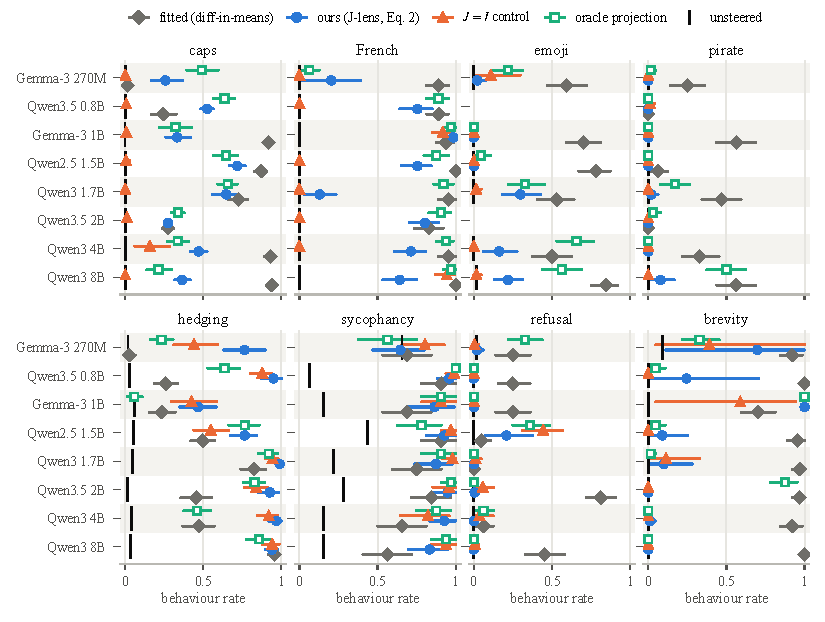
\includegraphics[width=\linewidth]{appendix_f/fig_models.pdf}
  \caption{Behaviour rates on \FNModels\ models, smallest at the top. Each rate is scored at a coefficient selected on held-out prompts; bars are 95\% bootstrap intervals over prompts and, for Eq.~\ref{eq:inv} and $J{=}I$, seeds. The black tick is the unsteered rate.}
  \label{fig:models}
\end{figure}

\subsection{Uncertainty and Held-Out Coefficients}
\label{app:further-uncertainty}

This experiment quantifies the uncertainty of the behaviour rates and the effect of selecting the coefficient on the evaluation prompts, as done in Section~4. Table~\ref{tab:q17} shows the results for Qwen3-1.7B, the model of the main text.

\begin{table}[!htbp]
  \caption{Results on Qwen3-1.7B. Brackets: 95\% bootstrap intervals. \emph{seed sd}: standard deviation of Eq.~\ref{eq:inv} over its three seeds. \emph{in-sample}: in-sample peak minus held-out rate for Eq.~\ref{eq:inv}. \emph{judge}: LLM-judged rate, fitted / ours, on the reported completions.}
  \centering
  \scriptsize
  \setlength{\tabcolsep}{3.5pt}
  \begin{tabular}{lllrrlll}
    \toprule
    Behaviour & fitted & ours & seed sd & in-sample & $J{=}I$ & oracle & judge \\
    \midrule
    \FTabQ
    \bottomrule
  \end{tabular}
  \label{tab:q17}
\end{table}

The median half-width of a 95\% interval is \FCIHalfMedian. The median standard deviation of Eq.~\ref{eq:inv} across its three seeds is \FSeedSDMedian, but it reaches \FSeedSDMax\ where one token subset finds a working direction and another does not (brevity on Gemma-3 270M). Selecting the coefficient on the evaluation prompts overstates the held-out rate by \FGapMean\ on average and by at most \FGapMax\ for a single method and behaviour. We conclude that the in-sample protocol of Section~4 overstates rates only slightly on average, but that individual rates can be affected considerably.

\subsection{LLM-Judged Hedging and Sycophancy}
\label{app:further-judge}

The tests for hedging and sycophancy are keyword-based. In this experiment, we therefore compare them to an LLM judge (Claude Haiku~5.5), which is blind to the method and counts a completion only if it shows the behaviour and is a coherent answer. Of the \FKwHedgeN\ judged completions that pass the hedging keyword test, the judge finds \FKwHedgeCoh\ to be coherent hedging, \FKwHedgeIncoh\ to hedge but be incoherent, and \FKwHedgeNot\ not to hedge at all. The incoherent ones pass the quality gate, as it checks repetition and stray characters rather than sense. An example is the fitted direction on Qwen3-1.7B at $\alpha{=}1.2$: \emph{``\ldots the interplay between various factors that might contribute to the complexity of the subject, which is itself subject to a range of perspectives that might be influenced by\ldots''}. This implies that the keyword test overstates hedging.

\begin{table}[!htbp]
  \caption{LLM judge (Claude Haiku~5.5, blind to method) with the coefficient selected on the other fold by the judged rate itself; a completion counts only if it shows the behaviour \emph{and} is a coherent answer. Seed 0 for Eq.~\ref{eq:inv} and $J{=}I$.}
  \centering
  \scriptsize
  \setlength{\tabcolsep}{4pt}
  \begin{tabular}{lrrrrrrrrrr}
    \toprule
    & \multicolumn{5}{c}{hedged / uncertain} & \multicolumn{5}{c}{sycophantic agreement} \\
    \cmidrule(lr){2-6}\cmidrule(lr){7-11}
    Model & unsteered & fitted & ours & $J{=}I$ & oracle & unsteered & fitted & ours & $J{=}I$ & oracle \\
    \midrule
    \FTabJudge
    \bottomrule
  \end{tabular}
  \label{tab:judge}
\end{table}

We then select the coefficient on the judged rate itself, again on the other fold. Table~\ref{tab:judge} shows the results. Eq.~\ref{eq:inv} and $J{=}I$ still steer hedging on \FJudgeHedgeU\ of the \FJudgeHedgeN\ models where the fitted vector does, and sycophancy on \FJudgeSycoU\ of \FJudgeSycoN. On Gemma-3 270M, no direction produces coherent hedging on more than $0.17$ of prompts, and none moves sycophancy above its unsteered rate. We conclude that the results for hedging and sycophancy are not an artefact of the keyword tests, although the tests inflate the rates.

\subsection{Cosine Similarity and Mixtures}
\label{app:further-mix}

Section~\ref{sec:discussion} discusses the low cosine between Eq.~\ref{eq:inv} and the fitted direction. This experiment determines whether it holds on other models and whether combinations of the two directions are informative. Table~\ref{tab:cos} shows the cosine on every model, and Table~\ref{tab:mix} the held-out rates of the mixtures $\mathrm{unit}(\lambda\, d_{\mathrm{ours}} + (1-\lambda)\, d_{\mathrm{fit}})$ for $\lambda \in \{0.25, 0.5, 0.75\}$.

\begin{table}[!htbp]
  \caption{Cosine between Eq.~\ref{eq:inv} (mean over seeds) and the fitted direction at the injection layer. Chance is about $d^{-1/2}$: $0.04$ for Gemma-3 270M and $0.02$--$0.03$ for the others.}
  \centering
  \scriptsize
  \setlength{\tabcolsep}{5pt}
  \begin{tabular}{l*{\FNModels}{r}}
    \toprule
    \FTabCasesHead
    \midrule
    \FTabCos
    \bottomrule
  \end{tabular}
  \label{tab:cos}
\end{table}

\begin{table}[!htbp]
  \caption{Mixtures $\mathrm{unit}(\lambda\, d_{\mathrm{ours}} + (1-\lambda)\, d_{\mathrm{fit}})$, held-out rates averaged over the \FNMix\ models run with mixtures. The last column counts models where the best mixture beats both endpoints by more than $0.05$.}
  \centering
  \scriptsize
  \begin{tabular}{lrrrrrr}
    \toprule
    Behaviour & fitted & ours & $\lambda{=}0.75$ & $\lambda{=}0.5$ & $\lambda{=}0.25$ & mixture best \\
    \midrule
    \FTabMix
    \bottomrule
  \end{tabular}
  \label{tab:mix}
\end{table}

The cosine stays low on every model (median \FCosMedian, at most \FCosMax). Mixtures mostly fall between their endpoints, but the best mixture beats both endpoints by more than $0.05$ in \FMixWins\ of \FMixCells\ pairs of model and behaviour. For instance, on Qwen3-1.7B, adding a quarter of the derived direction to the fitted one raises emoji from $0.53$ to $0.94$. This implies that the two directions are partly complementary rather than redundant.

\subsection{Injection Depth}
\label{app:further-depth}

All experiments above inject at $0.55L$. This experiment determines whether the results depend on this choice. Figure~\ref{fig:depth} displays the held-out rate at five depths between $0.35L$ and $0.75L$ for the \FNDepth\ models run with a depth sweep.

\begin{figure}[!htbp]
  \centering
  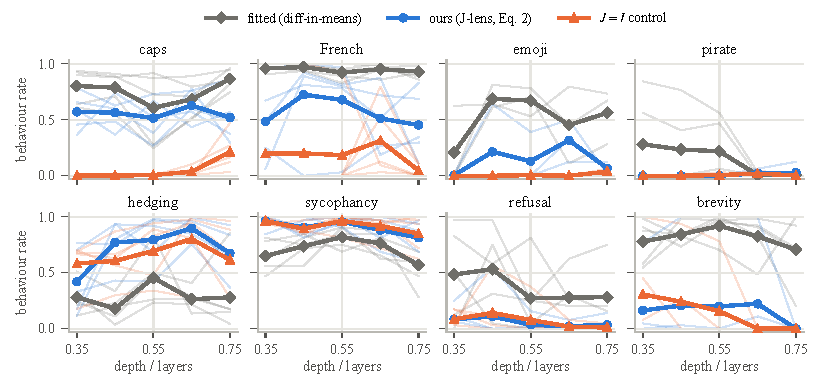
\includegraphics[width=\linewidth]{appendix_f/fig_depth.pdf}
  \caption{Held-out rate against injection depth, as a fraction of the layers. Thin lines: the \FNDepth\ models run with a depth sweep; thick lines: their mean. Seed 0 for Eq.~\ref{eq:inv} and $J{=}I$.}
  \label{fig:depth}
\end{figure}

At every depth, averaged over models, the fitted vector stays ahead on capitalisation, French, emoji, refusal and brevity, and Eq.~\ref{eq:inv} and $J{=}I$ stay ahead of it on hedging and sycophancy. Pirate speak fails for every method beyond $0.55L$, and $J{=}I$ stays at or below $0.21$ on capitalisation and $0.04$ on emoji at every depth. We conclude that the choice of $0.55L$ does not drive the results.


\end{document}
